\label{sec:NuMUCCsel}

\subsection{Event Selection and Muon Candidate Tagging}
\label{ssec:NuMUCCsel:sel}

\par The selection of $\nu_{\mu}$ events is built from the SliceID preselection (see sec. \ref{sec:sliceID:SliceID}) and a combination of cuts on slice-level and track-level observable values. The $\nu_{\mu}$ selection has this prescription: first, perform SliceID preselection; second, perform slice-level cuts to remove backgrounds; finally, perform track-level cuts to select one muon candidate.
\par Below is a summary of the variables used in this selection. There is some redundancy between this list and the list in sec. \ref{sec:NuMUCCsel:sel:vars}; this is intentional, as an overlap in phase space of the $\nu_{\mu}$ and $\nu_{e}$ selections improves constraining power.

\subsubsection{Variable Definitions}
\label{sssec:NuMUCCsel:sel:vars}

\par \noindent \textbf{Slice variables}: These variables generally describe the reconstructed neutrino interaction, i.e. the confluence of data gathered from all the PFParticles in the slice.
\begin{itemize}
    \item \emph{nslice}: number of neutrino slices identified by the SliceID (possible values are 0 or 1).
    \item \emph{n\_tracks\_contained}: number of tracks fully contained in the fiducial volume.
    \item \emph{reco\_nu\_vtx\_sce\_\{x,y,z\}}: Reconstructed, spacecharge-corrected neutrino interaction vertices in (x,y,z) coordinates (see fig. \ref{fig:numu_vtx}.
    \item \emph{topological\_score}: A machine-learned quantity that reflects the complexity and directionality of observable slice quantities. This variable has strong discriminating power between signal and cosmic-background (see \ref{fig:numu_topo_pid} (possible values are between 0 and 1).
    \item \emph{CRT Veto and Distance Tagger}: Tools provided by the cosmic ray tagger (see sec. \ref{sec:sliceID:CRT}).
\end{itemize}

\par \noindent \textbf{Track variables}: These variables specifically describe the reconstructed PFParticles; in interest to this selection are reconstructed track-like objects. 
\begin{itemize}
    \item \emph{trk\_sce\_\{start,end\}\_\{x,y,z\}}: Reconstructed, spacecharge-corrected start/end-points for the tracks.
    \item \emph{trk\_llr\_pid\_score}: The log likelihood ratio particle identification score (see sec. \ref{subsec:loglikelihoodpid}). This variable has strong muon-proton discriminating power (see fig. \ref{fig:numu_topo_pid}).
    \item \emph{trk\_score}: A machine-learned quantity that describes how `track-like' the reconstructed object is (possible values between 0 and 1).
    \item \emph{trk\_len}: The length of the reconstructed track (in cm).
    \item \emph{trk\_distance}: The distance from the start-point of the reconstructed track to the reconstructed neutrino vertex (in cm).
    \item \emph{pfp\_generation}: The generation of the PFParticle according to Pandora, i.e. how many parents the object on interest has in the slice.
\end{itemize}

\subsubsection{Backgrounds}
\label{sssec:NuMUCCsel:sel:bkgrnds}

\subsubsection{Event Selection}
\label{sssec:NuMUCCsel:sel:evt}

\par In this selection all slices must satisfy these criterion. The slice must be identified to be neutrino-like in nature, via SliceID, the topological score must be greater than 0.06, and the vertex must be in the fiducial volume of the detector. I.e:

\begin{itemize}
    \item \emph{nslice} = 1.
    \item \emph{n\_tracks\_contained} $>$= 1.
    \item \emph{reco\_nu\_vtx\_sce\_x} $\in$ [5,251] cm.
    \item \emph{reco\_nu\_vtx\_sce\_y} $\in$ [-110,110] cm.
    \item \emph{reco\_nu\_vtx\_sce\_z} $\in$ [20,986] cm.
    \item \emph{reco\_nu\_vtx\_sce\_z} $\not\in$ [675,775] cm.
    \item \emph{topological\_score} $>$ 0.06.
\end{itemize}

\par The final cuto on the $z$ coordinate is to ensure that it is not in the region of `dead wires' in the detector.

\par Run 3 has the additional power to leverage the CRT system and these cuts are additionally applied:

\begin{itemize}
    \item \emph{CRT Veto} != 1 or \emph{crthitpe} $<$ 100
    \item \emph{closestNuCosmicDist} > 5 cm
\end{itemize}

\subsubsection{Muon Selection}
\label{sssec:NuMUCCsel:sel:muonsel}

\par After the slice-level cuts are applied, the tracks in the slice are further analyzed to identify a muon candidate.

\begin{itemize}
    \item \emph{trk\_sce\_start\_x} $\in$ [5,251] cm.
    \item \emph{trk\_sce\_start\_y} $\in$ [-110,110] cm.
    \item \emph{trk\_sce\_start\_z} $\in$ [20,986] cm.
    \item \emph{trk\_sce\_end\_x} $\in$ [5,251] cm.
    \item \emph{trk\_sce\_end\_y} $\in$ [-110,110] cm.
    \item \emph{trk\_sce\_end\_z} $\in$ [20,986] cm.
    \item \emph{trk\_llr\_pid\_score} $>$ 0.2.
    \item \emph{trk\_trk\_score} $>$ 0.8.
    \item \emph{trk\_trk\_length} $>$ 10 cm.
    \item \emph{trk\_trk\_distance} $<$ 4 cm.
    \item \emph{pfp\_generation} = 2.
\end{itemize}

\begin{figure}
    \centering
    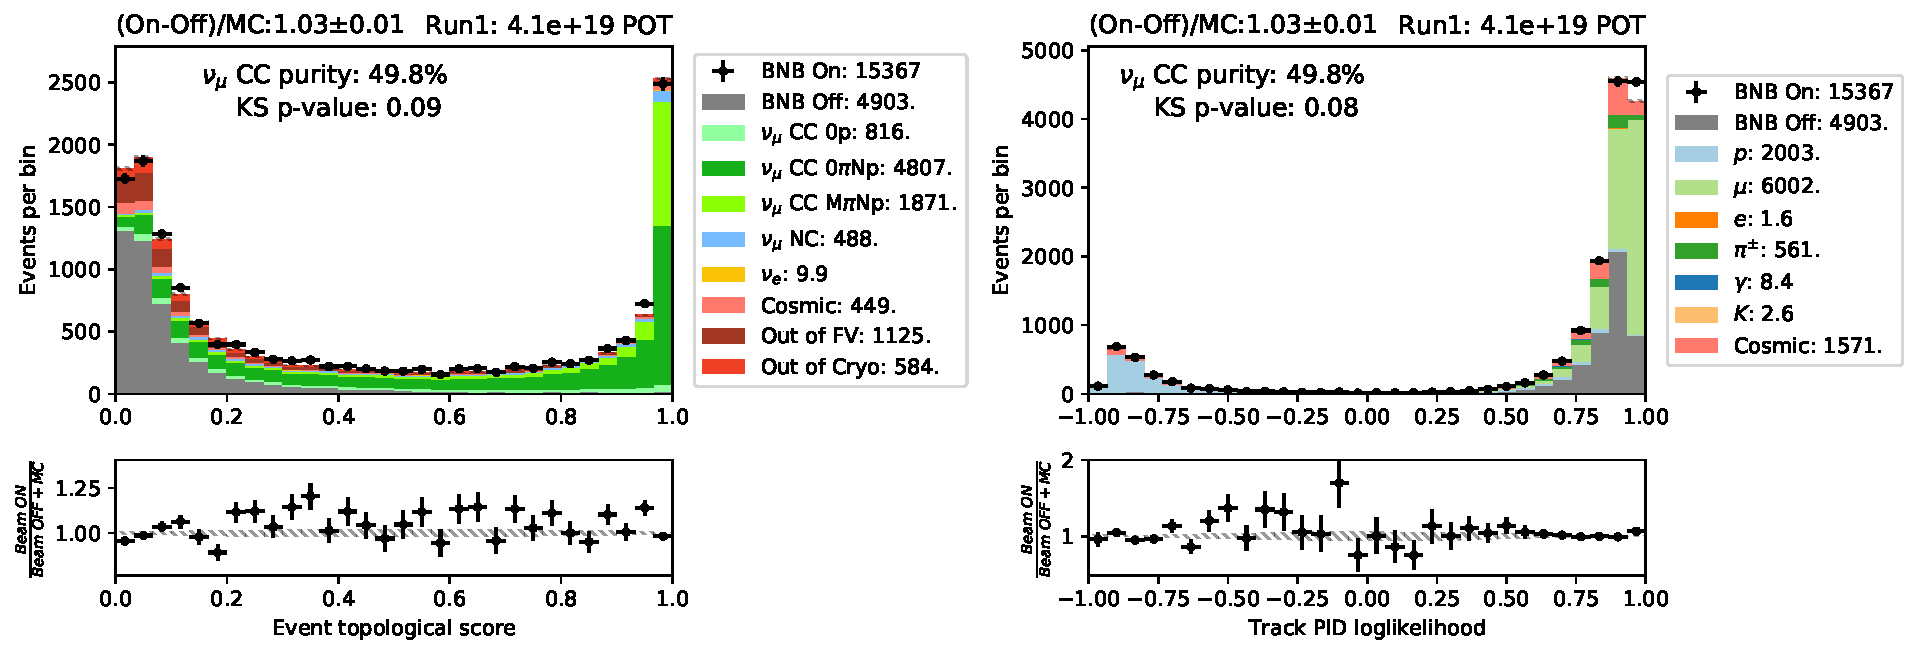
\includegraphics[width=\textwidth]{NuMuCCsel/Images/run1/numu_pret_run1.pdf}
    \caption{Caption}
    \label{fig:numu_topo_pid}
\end{figure}

\subsection{Inclusive Selection}
\label{ssec:NuMUCCsel:INC}

\subsubsection{Signal Definition}
\label{sssec:NuMUCCsel:INC:signaldef}
\par A $\nu_{\mu}$ event is identified by, at least, one muon candidate originating from inside the fiducial volume of the detector. Additional tracks and showers may accompany the muon candidate; these assist in the proper reconstruction of vertex location and energy calculation but are not necessary in the inclusive selection. 

\subsubsection{Run 1}
\label{sssec:NuMUCCsel:INC:Run1}
\par The first run of the MicroBooNE detector to employ the trigger system is known as `run 1' and includes data taken between February to July of 2016. Run 1 and run 3 (see sec. \ref{sssec:NuMUCCsel:INC:Run3} are two runs presented in this document. Run 1, being the older data-set, is more well-understood and also has a higher statistics than run 3. 



\begin{figure}
    \centering
    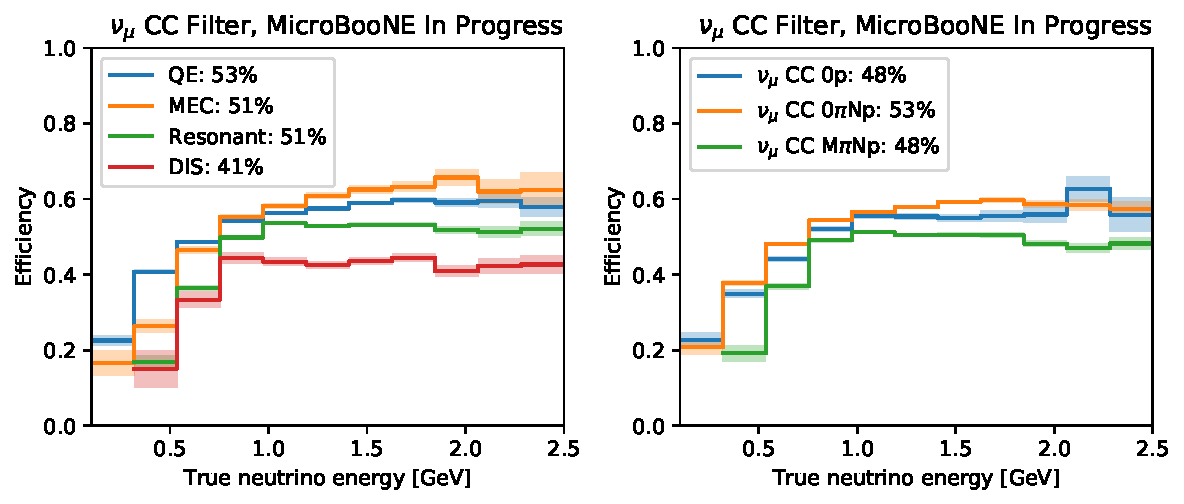
\includegraphics[width=0.85\textwidth]{NuMuCCsel/Images/run1/numu_efficiency_run1.pdf}
    \caption{Caption}
    \label{fig:numu_eff_r1}
\end{figure}

\begin{figure}
    \centering
    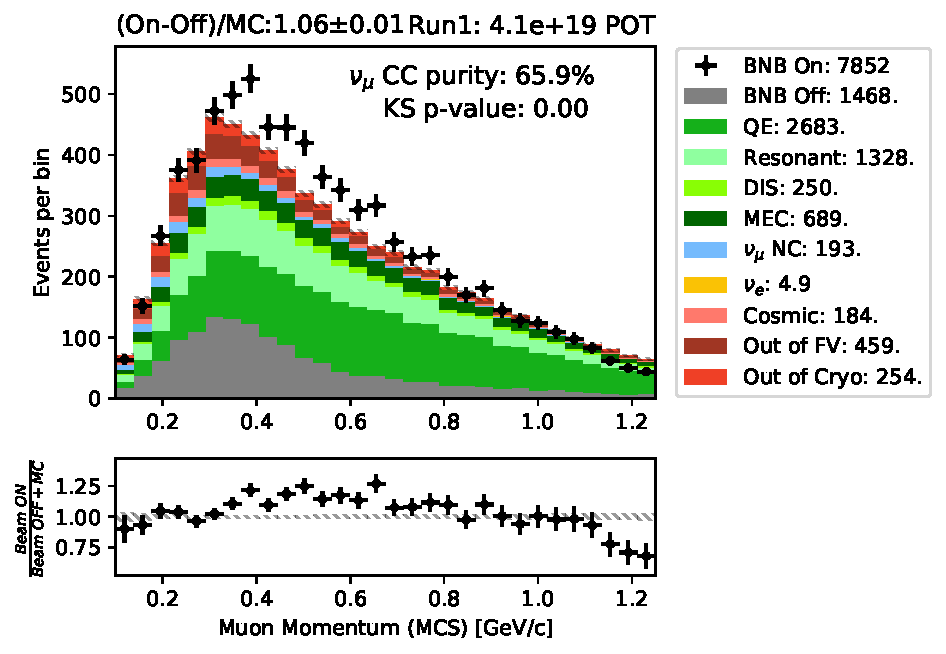
\includegraphics[width=0.495\textwidth]{NuMuCCsel/Images/run1/numu_mcsmom_run1.pdf} \hfill
    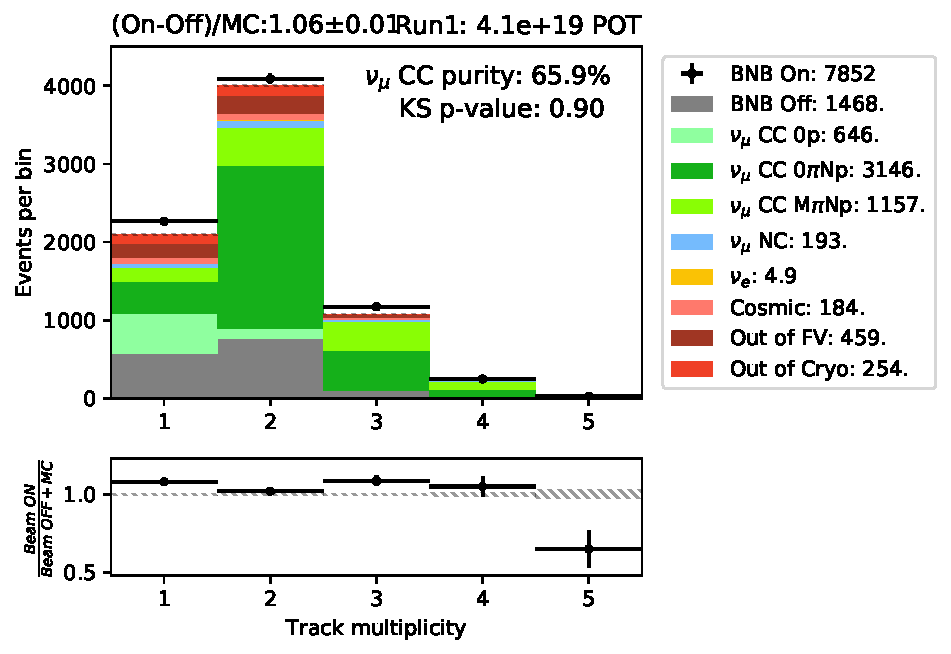
\includegraphics[width=0.495\textwidth]{NuMuCCsel/Images/run1/numu_vtxntrack_cat_run1.pdf}
    \caption{Caption}
    \label{fig:numu_mcs}
\end{figure}

\begin{figure}
    \centering
    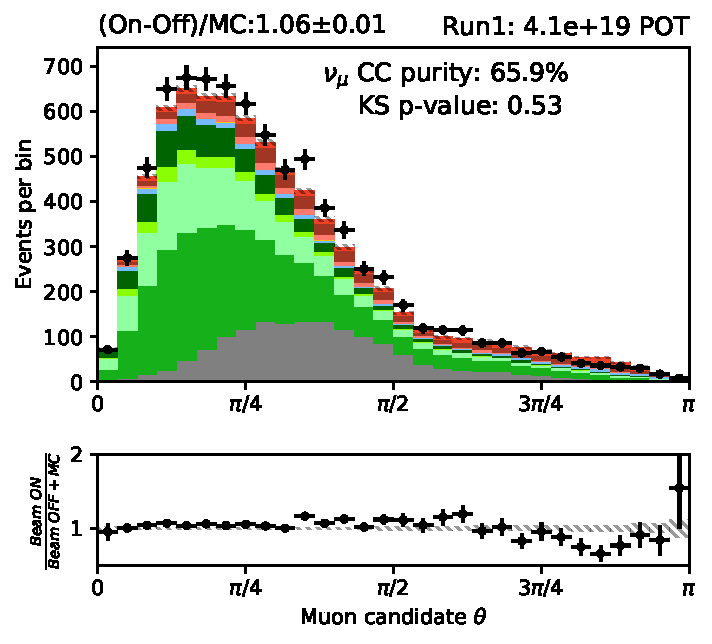
\includegraphics[height=6.5cm]{NuMuCCsel/Images/run1/numu_theta_run1.pdf} \hspace{2mm}
    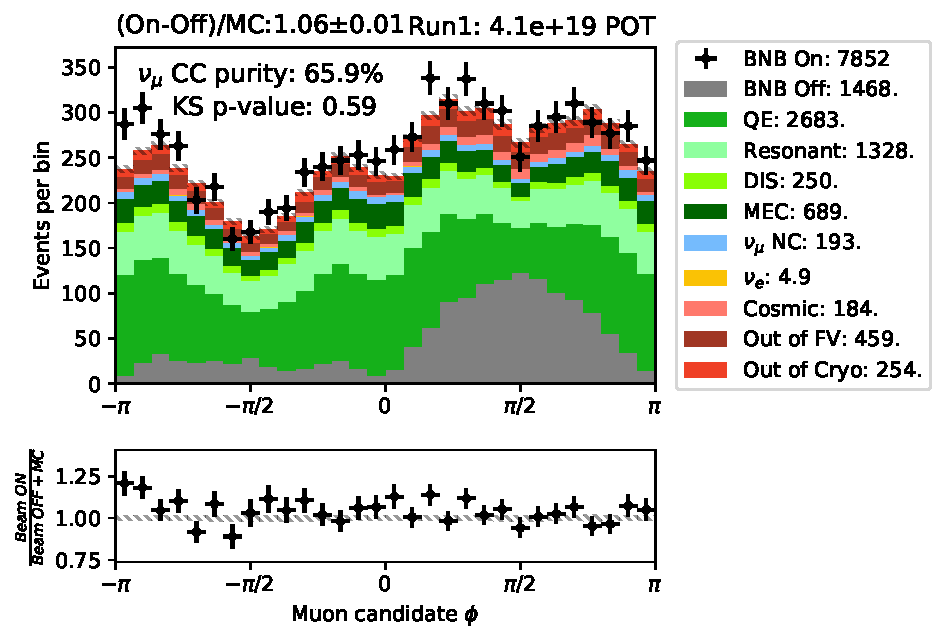
\includegraphics[height=6.5cm]{NuMuCCsel/Images/run1/numu_phi_run1.pdf}
    \caption{Caption}
    \label{fig:numu_angles}
\end{figure}

\begin{figure}
    \centering
    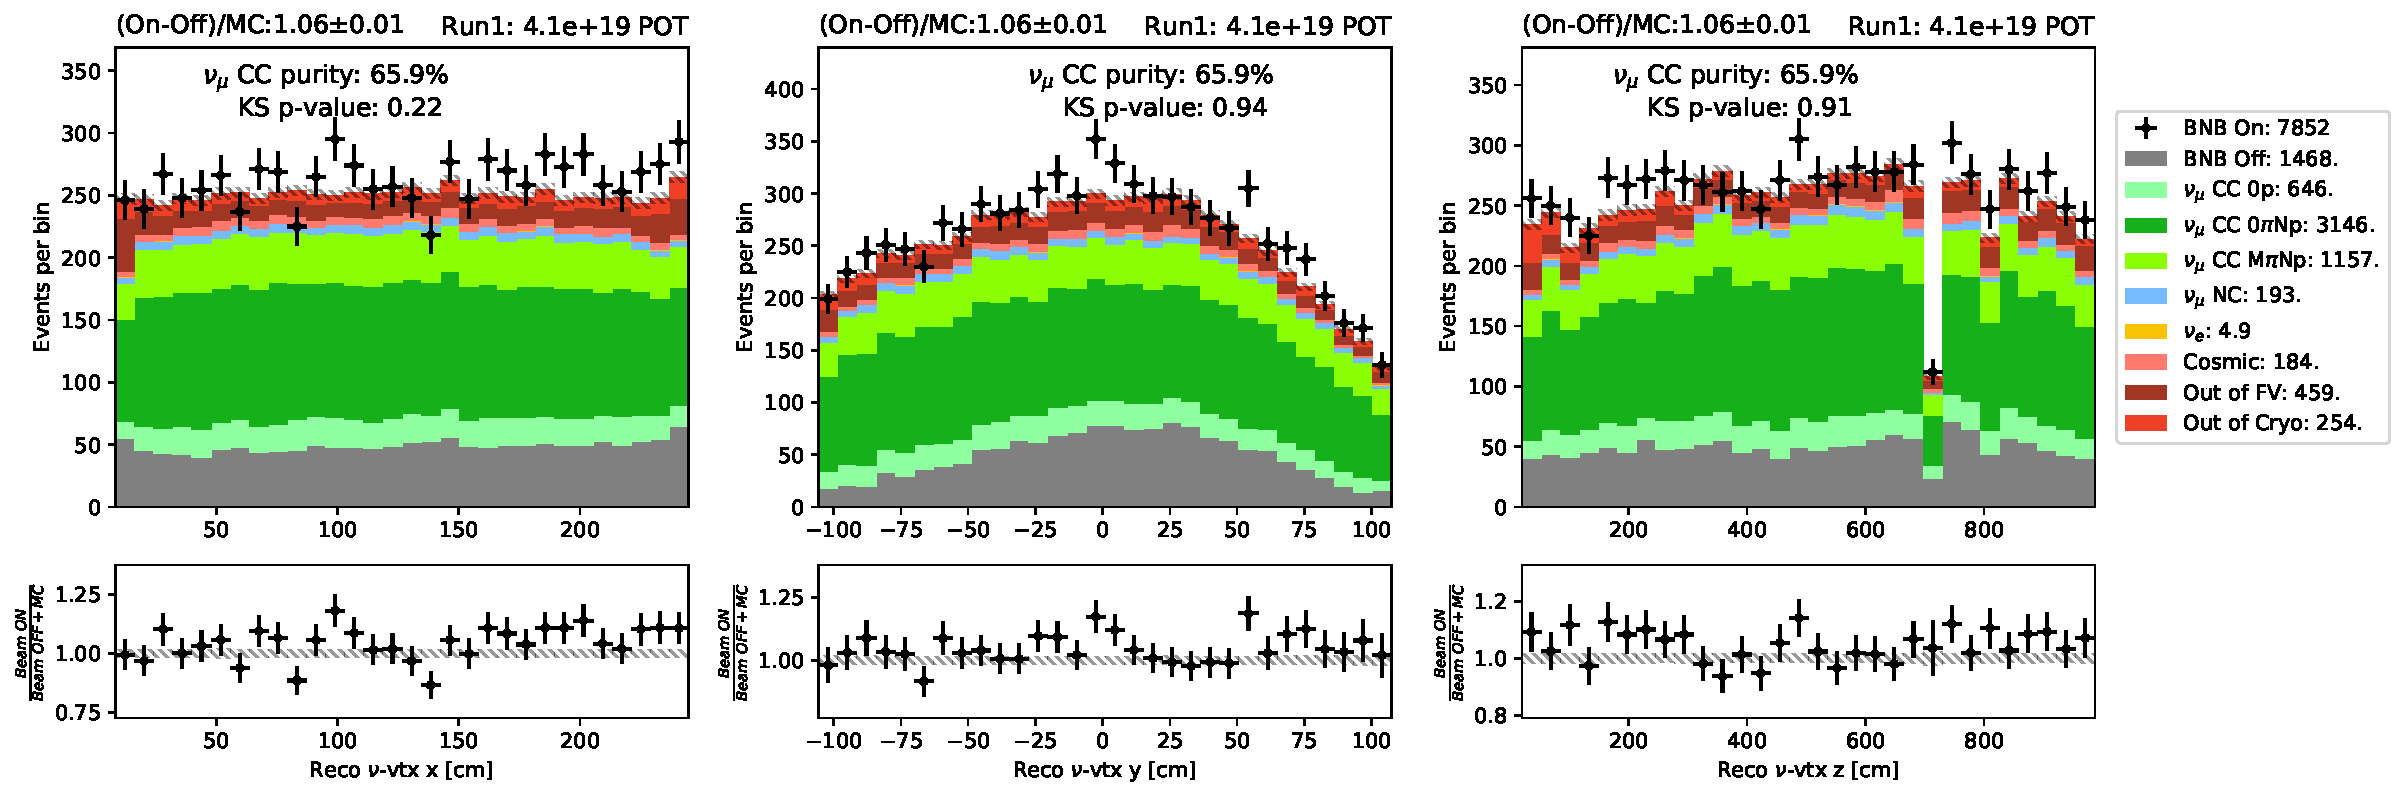
\includegraphics[width=\textwidth]{NuMuCCsel/Images/run1/numu_recovtx_run1.pdf}
    \caption{Caption}
    \label{fig:numu_vtx}
\end{figure}

\subsubsection{Run3}
\label{sssec:NuMUCCsel:INC:Run3}

\begin{figure}
    \centering
    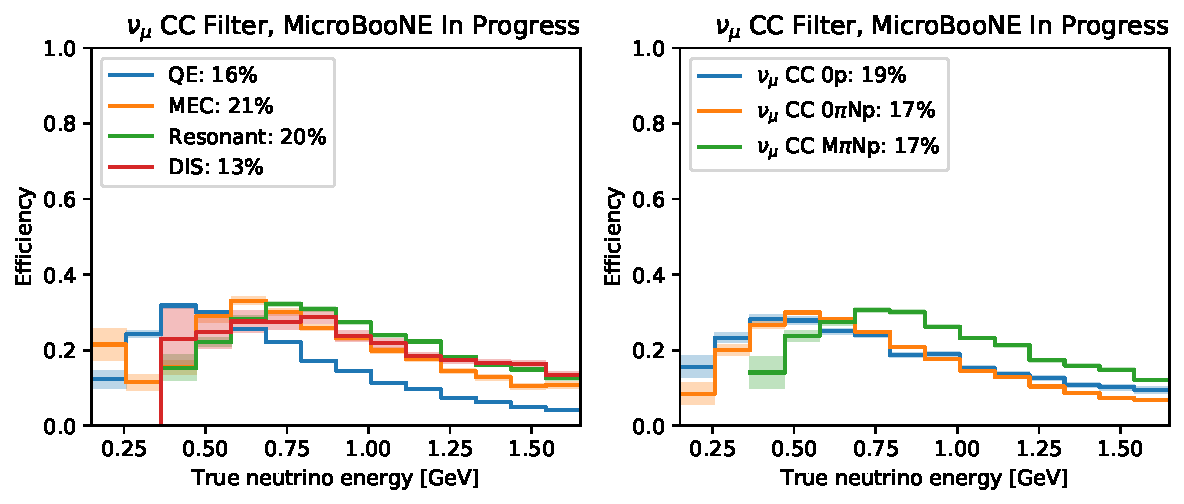
\includegraphics[width=0.85\textwidth]{NuMuCCsel/Images/run3/numu_efficiency_run3.pdf}
    \caption{Caption}
    \label{fig:numu_eff_r3}
\end{figure}


\begin{figure}
    \centering
    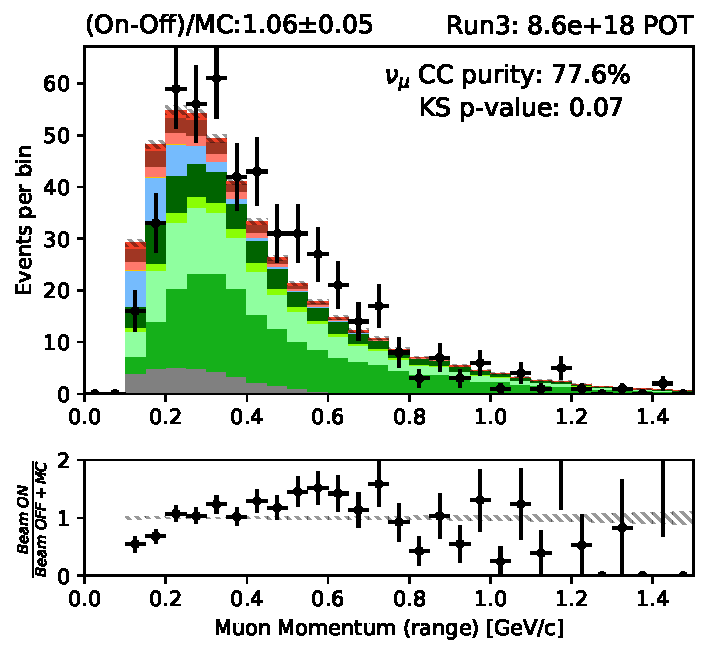
\includegraphics[height=6.5cm]{NuMuCCsel/Images/run3/numu_rangemom_run3.pdf} \hspace{2mm}
    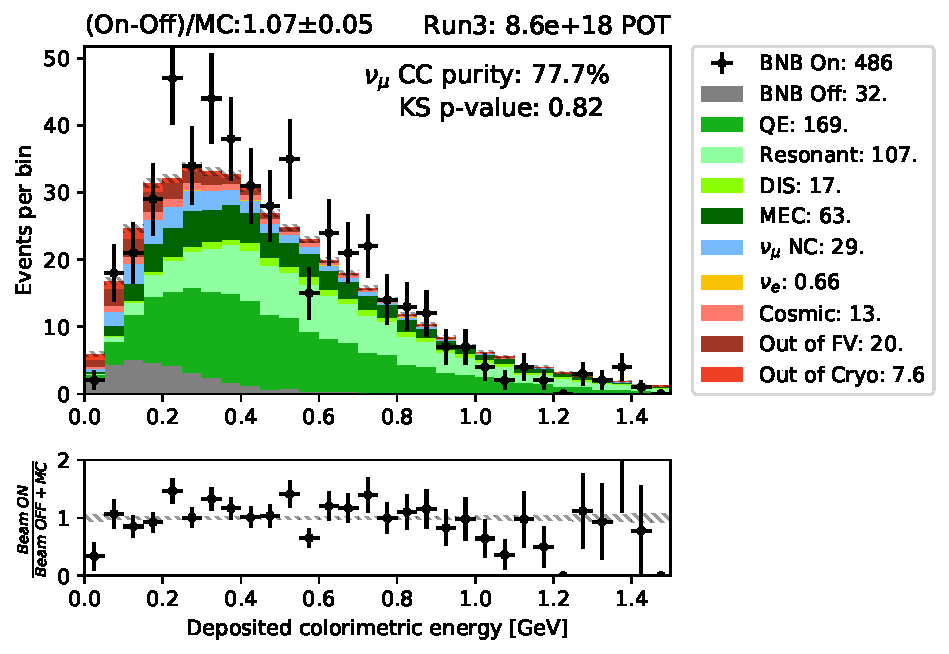
\includegraphics[height=6.5cm]{NuMuCCsel/Images/run3/numu_caloe_run3.pdf}
    \caption{Caption}
    \label{fig:numu_energy}
\end{figure}

\begin{figure}
    \centering
    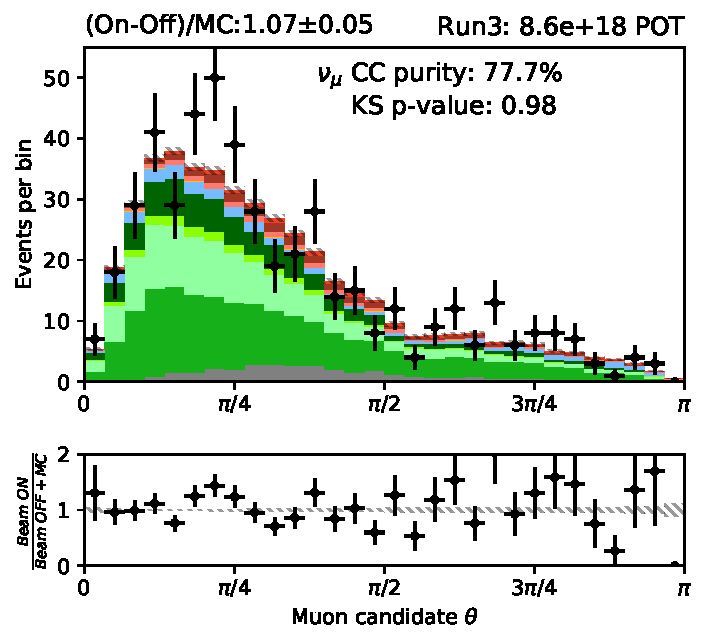
\includegraphics[height=6.5cm]{NuMuCCsel/Images/run3/numu_theta_run3.pdf} \hspace{2mm}
    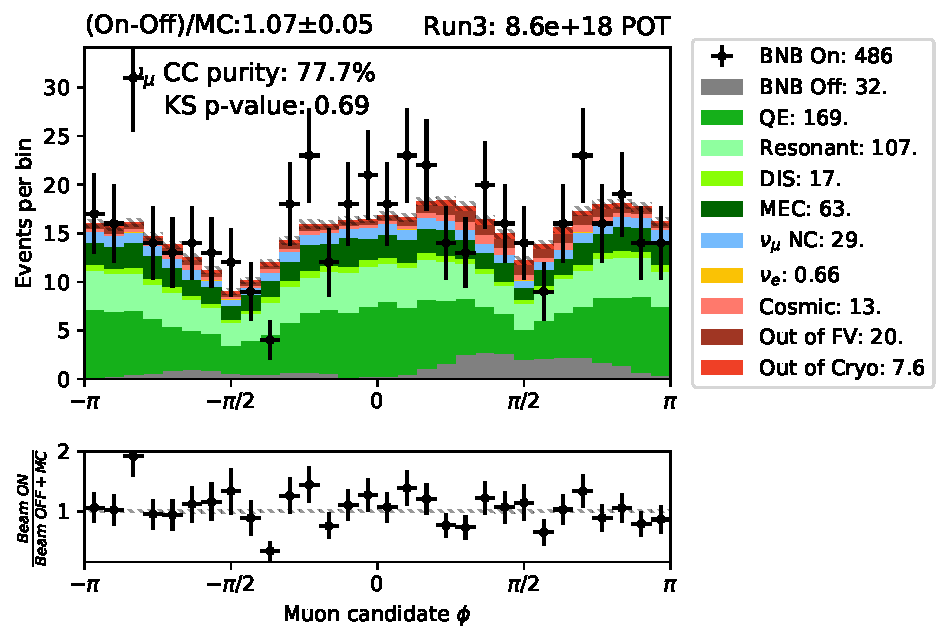
\includegraphics[height=6.5cm]{NuMuCCsel/Images/run3/numu_phi_run3.pdf}
    \caption{Caption}
    \label{fig:numu_angles}
\end{figure}
